\chapter{CPI Stacks for Vortex}

\Acrfull{cpi} stacks are a breakdown of the execution cycles into a set of classes. The breakdown aids in identifying potential bottlenecks in the architecture. In my project thesis~\cite{Aurud_Project}, I implemented a \acrfull{rtl} solution to create \acrshort{cpi} stacks for \Gls{vortex} (CSV). My solution utilized a classification scheme based on \acrshort{gsi}~\cite{GSI_GPU_Stall_Inspector} which will be described in the next section. Section~\ref{sec:csv} will then briefly describe how my implementation of \acrshort{csv} differs from \acrshort{gsi}, and Section~\ref{sec:improve_csv} will describe how I improved \acrshort{csv} in this thesis.

\section{GPU Stall Inspector} \label{sec:gsi}

The \acrfull{gsi}~\cite{GSI_GPU_Stall_Inspector} is a stall attribution tool that enables detailed classification of memory stalls. They also present a set of classes for instruction stalls, which is also used by GCoM~\cite{gcom}. \acrshort{gsi}'s classification is done in two separate steps. First, if no warps are issued, a stall type is attributed to each warp in the issue stage. The attribution is done based on the cause most strongly preventing execution, i.e. the stall cause most likely to remain in the next cycle. The details regarding the priority can be found in the \acrshort{gsi} paper~\cite{GSI_GPU_Stall_Inspector}. Once each warp is classified, the issue cycle is classified based on the inverse priority\footnote{The priority is not exactly inversed, as memory and synchronization stalls are prioritized over compute stalls in
both steps.} of the stalled warps, i.e. the cause of the warp which is least likely to continue stalling in the next cycle.

\vspace{1mm}\noindent
Following is a list describing the classes used by \acrshort{gsi}:

\begin{itemize}
    \item \textbf{Base}: If any of the warps are issued, the cycle is a base cycle.
    \item \textbf{Idle}: The warp is not active, indicating that the kernel is not fully utilizing the GPU, because of poor load balancing or because there is not enough work.
    \item \textbf{Control stall}: The warp instruction supplied by the instruction buffer is not the next instruction to be executed by the warp. This might be due to a high degree of divergence in the kernel.
    \item \textbf{Synchronization stall}: The warp is blocked due to a barrier, to synchronize with other warps.
    \item \textbf{Memory data stall}: The warp cannot issue because the operands are dependent on the result of a pending load.
    \item \textbf{Memory structural stall}: The warp is a memory instruction requiring the \acrshort{lsu}, but it cannot be issued because the \acrshort{lsu} is not ready.
    \item \textbf{Compute data stall}: The warp cannot issue because the operands are dependent on the result of a pending compute instruction. Compute instruction refers to every non-memory instruction. 
    \item \textbf{Compute structural stall}: The warp is a compute instruction, but the required functional unit is not ready.
\end{itemize}

%\textcolor{red}{\acrshort{gsi} has some issues: Does not give a full view of the issue stage (are multiple warps stalled? What are the cause of this, how many warps can be cannot be scheduled etc.)}

\section{CSV Overview} \label{sec:csv}

This section describes how I adapted the \acrshort{gsi} classification scheme in my project thesis~\cite{Aurud_Project}, to create \acrshort{csv}. As the baseline version of \Gls{vortex} only selects one warp to attempt to issue, the two step scheme of \acrshort{gsi} was not required. Instead, \acrshort{csv} only sampled the stall cause of the warp selected by \Gls{vortex}' issue scheduler. Every cycle, each \acrshort{sm} attributes its cycle to the class corresponding with its stall cause. Later, the data from each \acrshort{sm} is read and accumulated to create the results for the entire \acrshort{gpu}.

When a data stall occurs, the functional unit or combination of functional units, which reserved the operand register(s), are used to track the type of data stall. If both of the operands are reserved, half of the cycle is attributed to each of the sources. For example, if a warp is waiting for results from both the \acrshort{alu} and the \acrshort{lsu}, one half of the cycle is attributed as a \textit{memory data} stall and the other half is attributed as a \textit{memory structural} stall. 

To simplify the implementation, I grouped \textit{control} and \textit{synchronization} stalls into one class: \textit{sync \& control}. \textit{Sync \& control} stalls occur if there are no warps in the instruction buffer, and there are no ready warps in fetch's warp scheduler. Additionally, I included a class for \textit{empty ibuffer} which occurs if there are no warps in the instruction buffer but there are ready warps in the warp scheduler. This could occur if there is significant latency between fetching an instruction and it being available in the instruction buffer.

An issue with sampling \textit{idle} stalls is that the \acrshortpl{sm} terminate at different times. The \acrshortpl{sm} will therefore not be able to track idle cycles after completing, while other \acrshortpl{sm} continue execution. The idle cycles can thus not be read by the \acrshortpl{sm} themselves. To solve this, the number of idle cycles can instead be calculated as

\begin{equation} \label{eq:idle}
    C^i_{idle} = \textrm{max}(C^i_{active}) - C^i_{active}
\end{equation}
\noindent
where $\textrm{max}(C_{active})$ represents the number of cycles used to run the program, and $C^i_{active}$ represents the number of active cycles for the $i$th \acrshort{sm}.

While the \textit{data} and \textit{structural} stalls described by \acrshort{gsi} can occur individually, an instruction can also be stalled by both at the same time. This is why I included a \textit{data \& structural} stall class. If a warp is waiting for both data and the functional unit to be ready, it would thus be attributed to a separate class rather than having to prioritize one class over another.

\section{Improving CSV} \label{sec:improve_csv}

As I see it, \acrshort{gsi} and the version of \acrshort{csv} implemented in my project thesis has a key weakness: it does not describe the entire state of the issue stage. For example, if multiple warps are available, and all are memory structural stalls except one compute structural stalled warp, the cycle will be classified as compute structural stall. This may mislead us into thinking that the throughput of the compute functional units is the bottleneck. Resolving the 'issue' would just reveal the cause of all the other warps. Another example would be a case where the GPU frontend does not fetch enough instructions. This would result in many data stalls, due to having a small selection of warps in the issue stage. However, the real problem might be control or synchronization stalls. As the classification is not proportional to the number of each stall cause, the solutions will not lead to a proportional change. It will also be hard to say if the proposed solutions just revealed existing stalls or actually caused new behaviour. 

\begin{figure}
     \centering
     \begin{subfigure}[t]{0.45\textwidth}
         \centering
         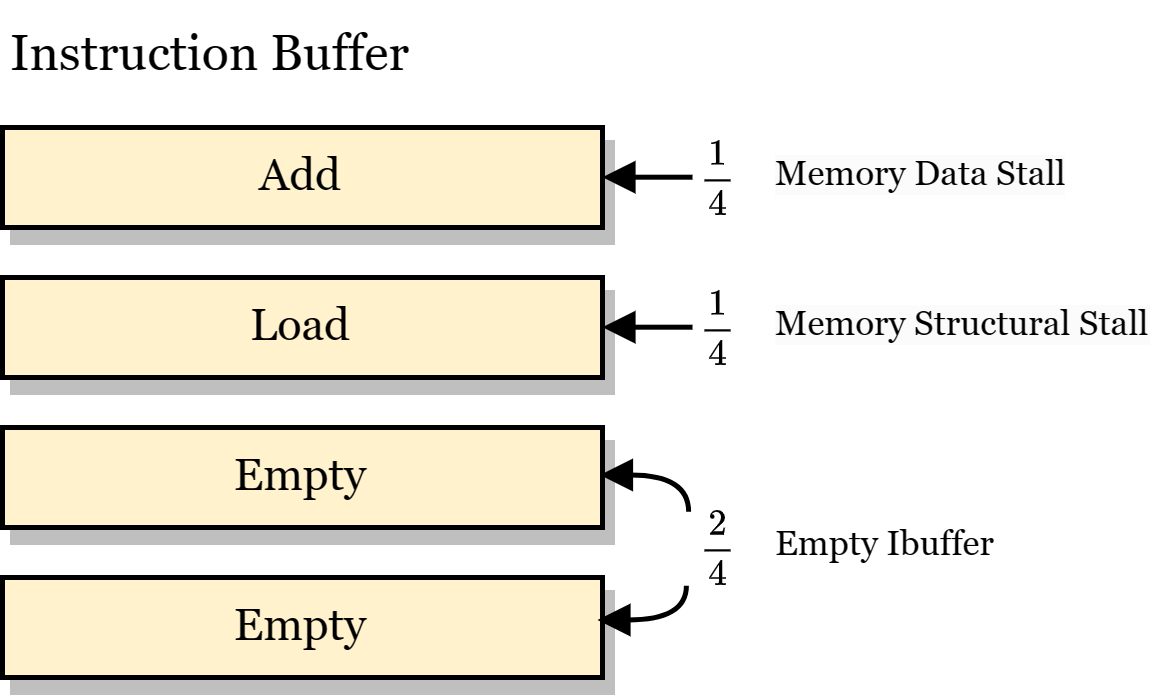
\includegraphics[width=\textwidth]{figures/proportional-stall-ex1.png}
         \caption{The add instruction is waiting for the result of a load. The load is waiting for the LSU to be ready while the two remaining buffers are empty}
         \label{fig:prop_stall_1}
     \end{subfigure}
     \hfill
     \begin{subfigure}[t]{0.45\textwidth}
         \centering
         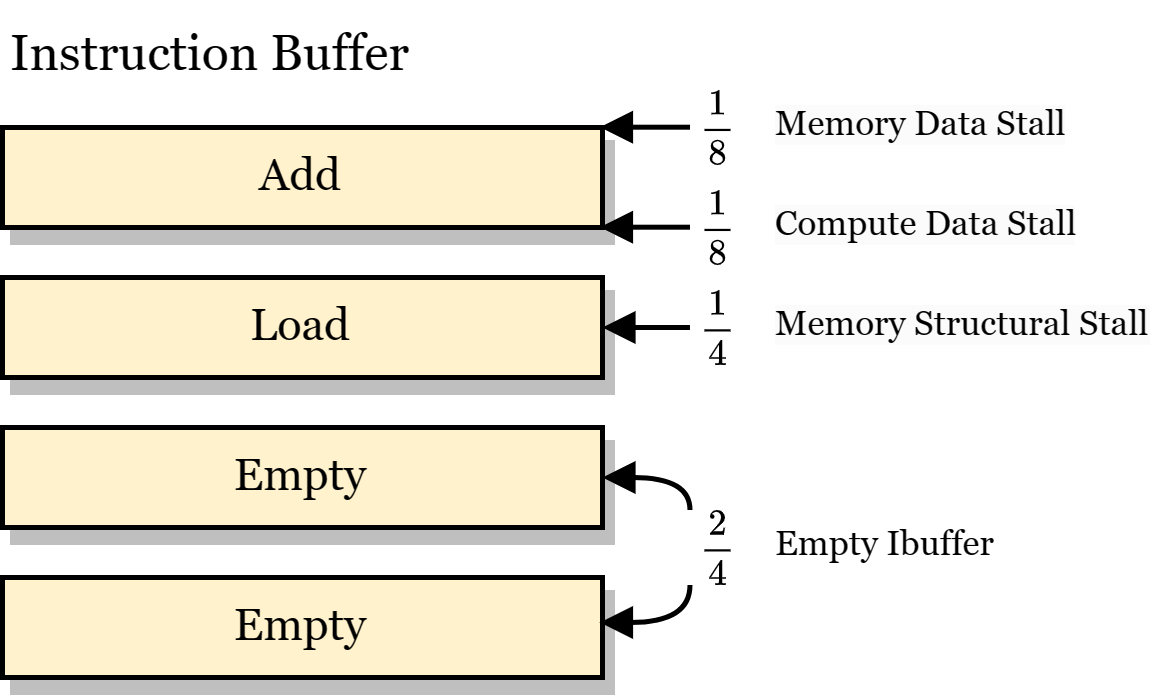
\includegraphics[width=\textwidth]{figures/proportional-stall-ex2.png}
         \caption{The add instruction is waiting for the result of a load and a computation. The load is waiting for the LSU to be ready while the two remaining buffers are empty}
         \label{fig:prop_stall_2}
     \end{subfigure}
        \caption{Examples of TIP-inspired stall classification with 4 warps in an \acrshort{sm}.}
        \label{fig:lrr-gto}
\end{figure}

To resolve this weakness I took inspiration from TIP~\cite{TIP} to get a better overview of why warps stall. When a stall occurs, all warps in the \acrshort{sm} attribute the cause(s) of their stall. Then $1/N$th of the cycle is attributed to the stall class of each warp, where $N$ represents the number of warps per \acrshort{sm}. Figure~\ref{fig:prop_stall_1} shows an example of how the cycles may be attributed. If a warp has multiple causes for stalling, i.e. a combination of data stalls and/or a structural stall, the $1/N$th cycle is further divided evenly among the stalls, as illustrated in Figure~\ref{fig:prop_stall_2}. By doing this, the \textit{data \& structural} can be removed, as the causes will be attributed proportionally. By attributing the cycles in proportion to the occurrence of the stalls, we get a better overview of the entire issue stage and why no warp can be issued. 

With my new attribution scheme, I have to include an additional stall class: \textit{missed schedule}. This is required as the baseline instruction scheduler might stall due to selecting a stalling warp, while a ready warp is available. In this case, the ready warps are attributed as \textit{missed schedule}. Figure \ref{fig:cpi_flowchart} shows a flowchart for how the cycles are attributed.

\begin{figure}
    \centering
    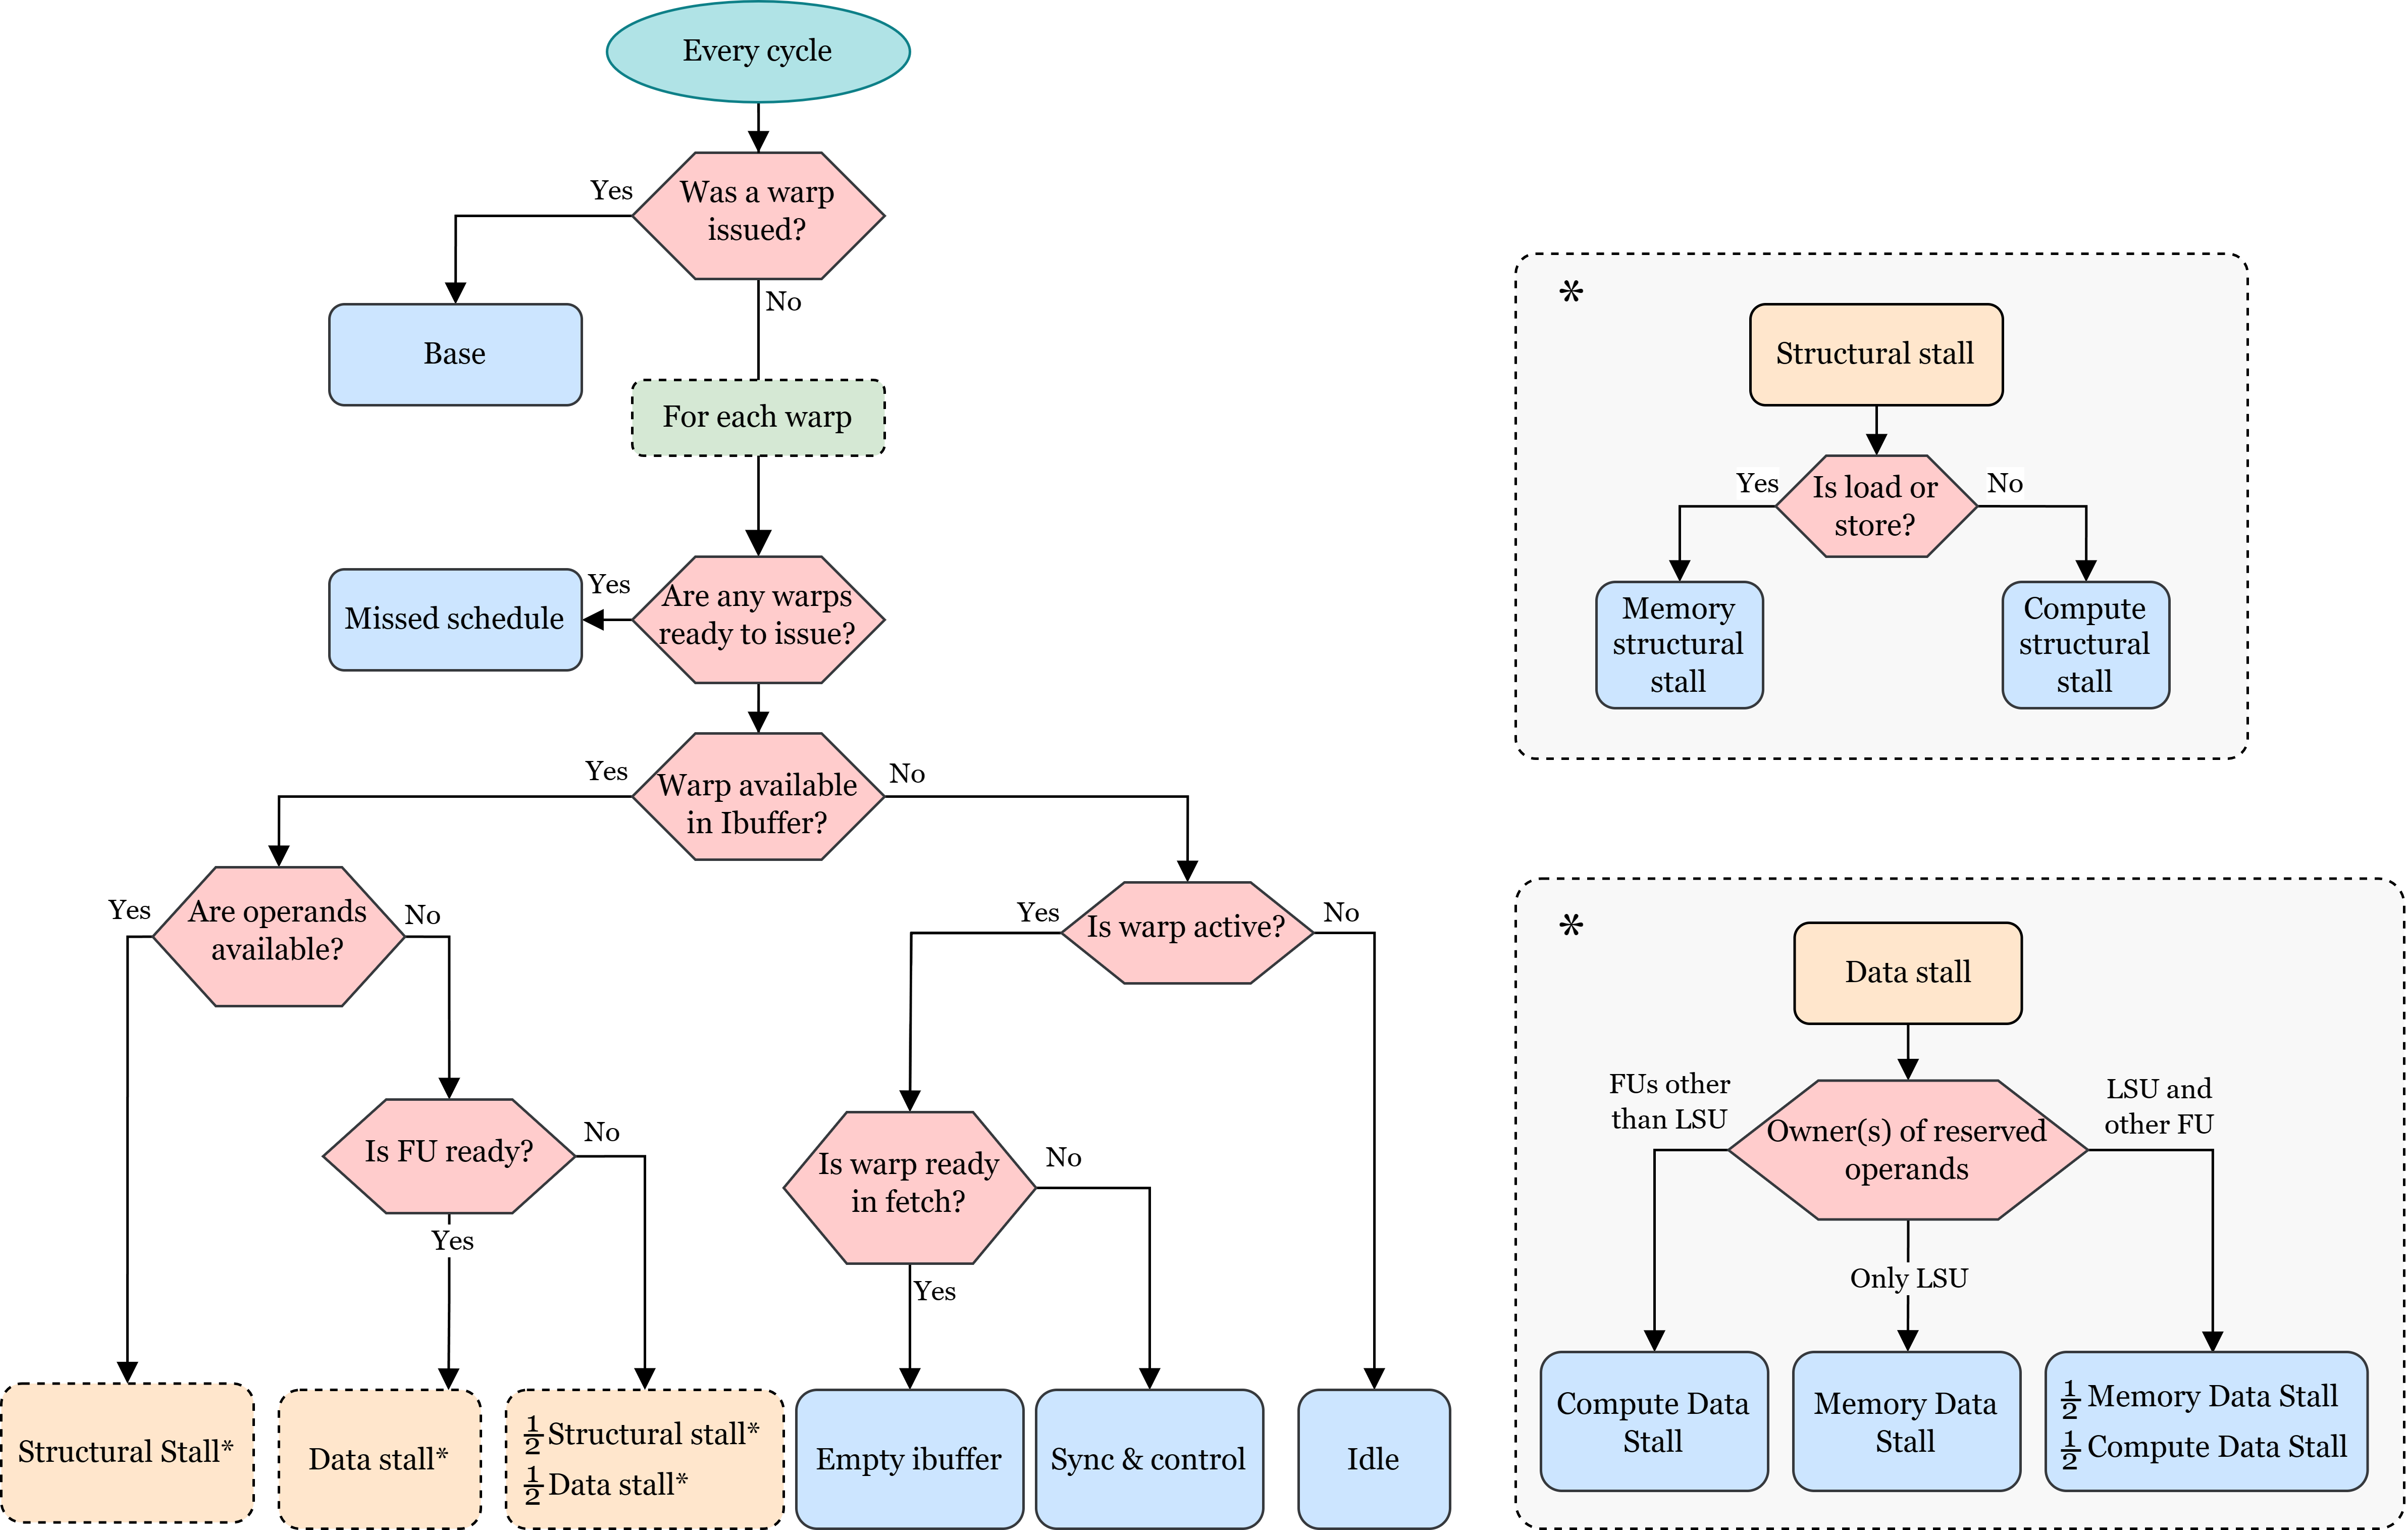
\includegraphics[width=\textwidth]{figures/flowchart_grouped_v2.png}
    \caption[Flowchart for \acrshort{csv}'s cycle attribution.]{Flowchart for \acrshort{csv}'s cycle attribution. Data and structural stalls are divided if they occur together. Data stalls may also be further divided if an instruction is waiting for results from both memory and compute.}
    \label{fig:cpi_flowchart}
\end{figure}